% Modern editorial, markup and figure/layout contributions: CC-BY-SA-4.0.
% Historical text and illustrations: Leonhard Euler (1744), public domain.
% Component scope and upstream attribution: see RIGHTS.md.
% Vector redraw: Tabula I, Fig. 2. Equal abscissa intervals retained.
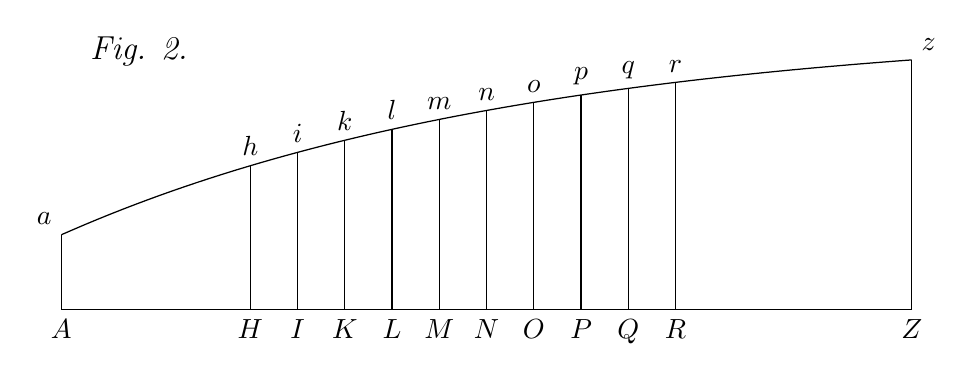
\begin{tikzpicture}[x=1.2cm,y=.95cm,line width=.45pt]
\draw (0,1)--(0,0)--(9,0)--(9,{1+2.8*(1-exp(-9/5))});
\draw[domain=0:9,samples=70] plot (\x,{1+2.8*(1-exp(-\x/5))});
\foreach \X/\U/\L in {2/H/h,2.5/I/i,3/K/k,3.5/L/l,4/M/m,4.5/N/n,5/O/o,5.5/P/p,6/Q/q,6.5/R/r}{
\draw (\X,0)--(\X,{1+2.8*(1-exp(-\X/5))});
\node[below] at (\X,0) {$\U$};
\node[above] at (\X,{1+2.8*(1-exp(-\X/5))}) {$\L$};}
\node[below] at (0,0) {$A$};\node[above left] at (0,1) {$a$};
\node[below] at (9,0) {$Z$};\node[above right] at (9,{1+2.8*(1-exp(-9/5))}) {$z$};
\node[anchor=west] at (.2,3.45) {\large\textit{Fig. 2.}};
\end{tikzpicture}
